%The LHC and ATLAS are explained
%MC needs to be explained, how are systematics displayed
%DR and DS needs to be explained in the context of ATLAS


\chapter{The LHC and the ATLAS detector}
\label{lhc_atlas}


For most researches in modern particle physics there are two main constraints. The first one arises from the statistical nature of decay and creation processes in particle physics. Many of the most interesting events occur extremely rarely and call for large amount of data or more precisely high luminosity, to achieve statistically significant results. Secondly the energy scale of particle physics is enormously high and therefore the energy needed to allow breaking the structure of particles below the nuclear scale. 

This work was carried out using simulations based on the ATLAS~\cite{atlas} detector at the Large Hadron Collider (LHC)~\cite{lhc_machine} which offers both a record breaking center-of-mass energy and luminosity. This chapter summarises both machines and provides the knowledge necessary to understand the simulations used. First of all, a summary of the machines' parts and their technical details is given, followed by a description of how the detector detects particles and how their properties are measured. Simulations of detector events are explained and the event selection for this work is covered.

\section{Large Hadron Collider}

The Large Hadron Collider, located at the facilities of the European Organization of Nuclear Research (CERN) close to Geneva, was built to extend the frontiers of modern particle physics by delivering high luminosities and reaching unprecedented high energies thereby providing the data benefitting multiple particle physics experiments.

The LHC is a circular particle collider with a circumference of \SI{26.7}{\kilo \metre} designed to  accelerate and collide two counter-rotating proton beams. The protons are accelerated in bunches of up to \num{d11} protons at  energies up to \SI{6.5}{\tera \electronvolt} and a luminosity of \SI{d34}{\per\square\cm \per\s}, achieving the record center-of-mass energy of up to \SI{13}{\tera \electronvolt}. The bunches are pre-accelerated by a number of accelerators before being inserted in the last, so called, storage ring. An overview of the acceleration system is given in figure \ref{fig:accelerator_complex} and for more detailed information one can refer to the LHC design report.~\cite{lhc_machine}. 
The four main interaction points, at which the beams are brought to collision, contain the main experiments of the LHC. Two of them are general purpose detectors, namely ATLAS~\cite{atlas} and CMS.~\cite{cms} The third is the LHCb~\cite{lhcb} which focuses on bottom-quark physics. Lastly, ALICE~\cite{alice} is used for investigating heavy ion collisions. Figure \ref{fig:LHC} shows a sketch of the LHC's location and the positions of the four main experiments.

\begin{figure}[htbp]
\centering
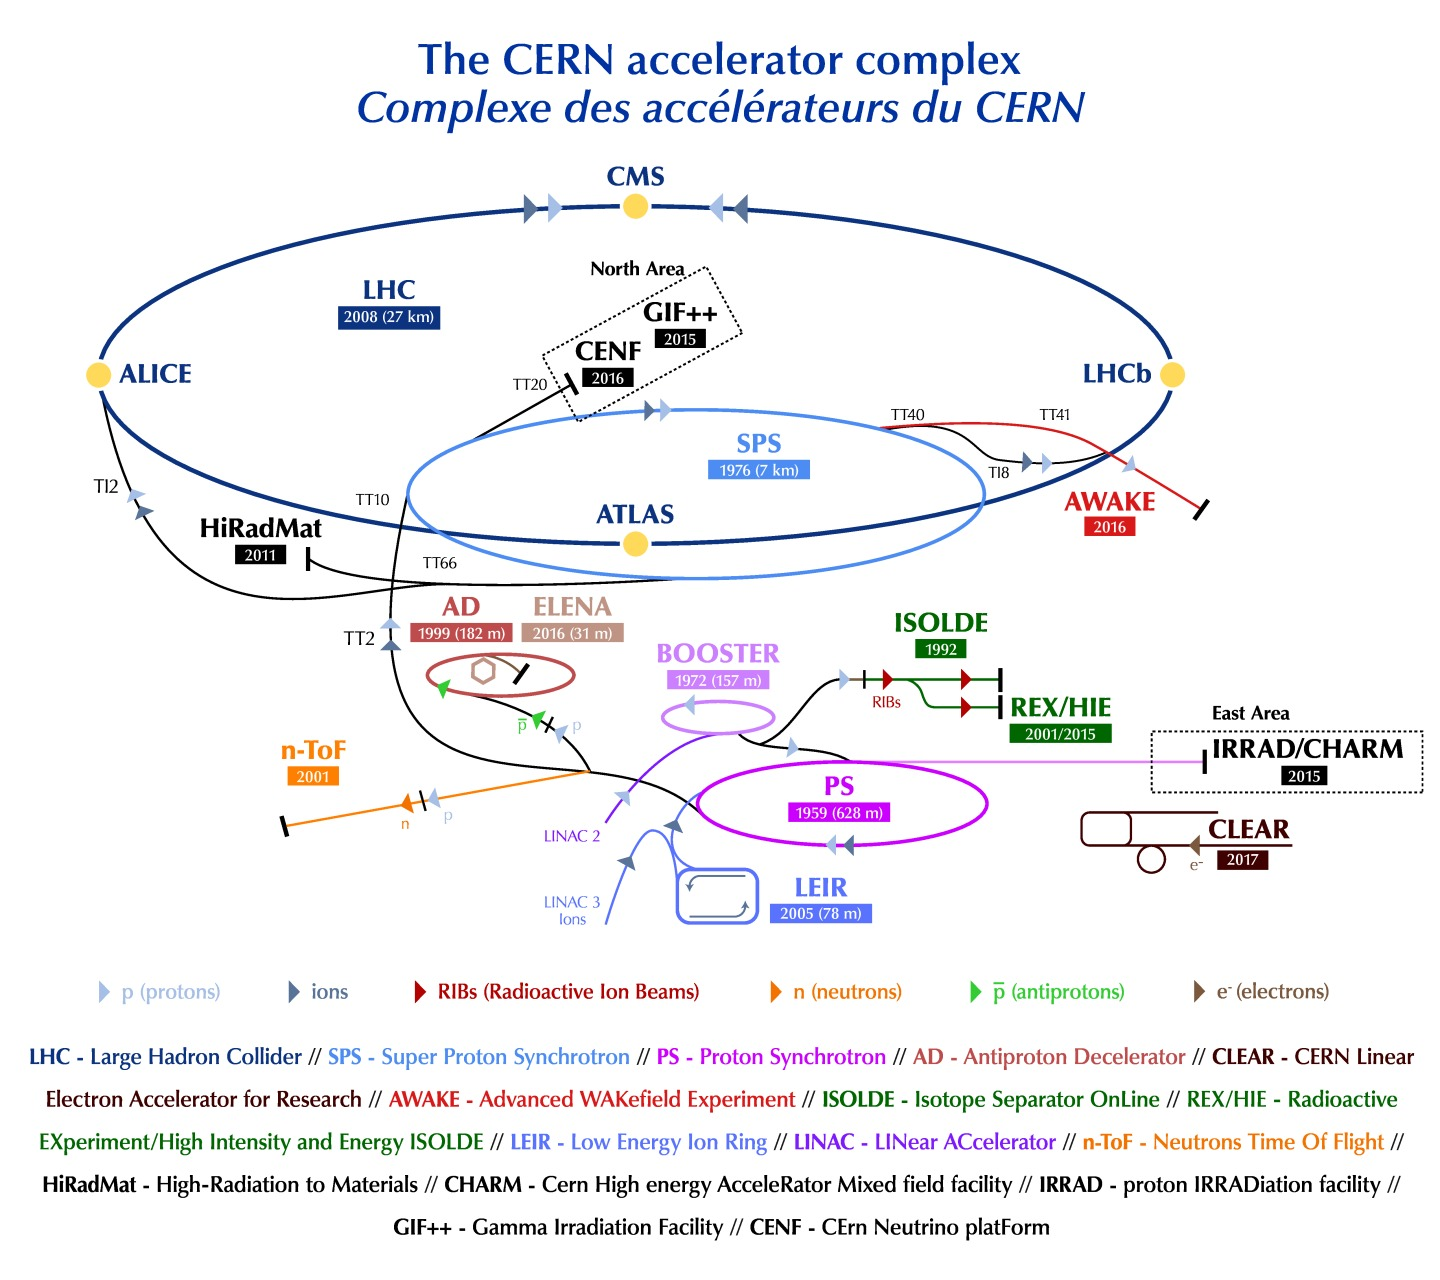
\includegraphics[width=\figwidth]{figures_LHC/CCC-v2018-print-v2.jpg}
\caption[Sketch of the LHC accelerator complex]{Sketch of the LHC accelerator complex showing the acceleration systems and the main storage ring with its experiments.~\cite{Mobs:2636343}}
\label{fig:accelerator_complex}
\end{figure}

\begin{figure}[htbp]
  \centering
  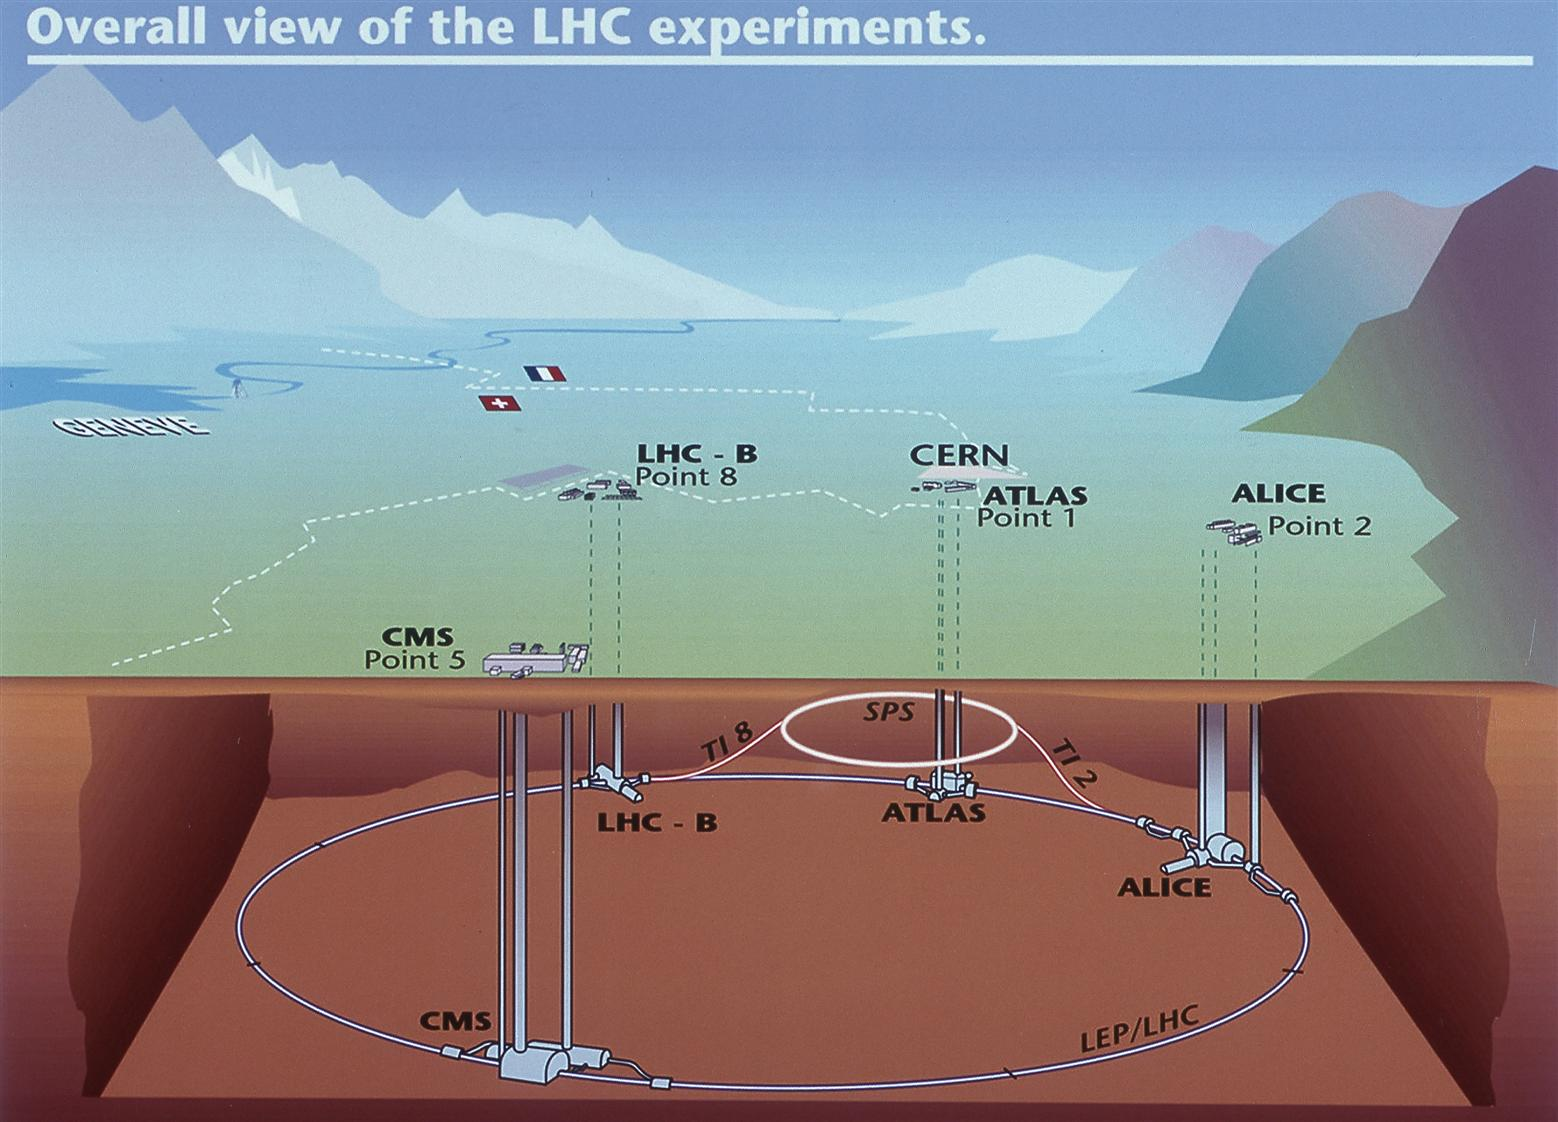
\includegraphics[scale=0.4]{figures_LHC/CERN-all-experiments.jpg}
  \caption[Sketch of the LHC ring.]{Sketch of the LHC ring, the position
    of the experiments and the surrounding countryside. The four big
    LHC experiments are indicated (ATLAS, CMS, LHC-B and ALICE) along with their injection lines (Point 1, 2, 4, 8).~\cite{Jean-Luc:841555}}
  \label{fig:LHC}
\end{figure}


\section{The ATLAS detector}

The ATLAS detector is a general purpose detector meaning it aims at covering a maximum number of final states, enabling reasearchers in may topics of particle physics to use its data.

ATLAS, \enquote{A Toroidal LHC Apparatus} has the distinguishing structure of a general purpose detector, its innermost part formed by tracking detectors directly surrounding the interaction point, followed by calorimeters, and a final layer for muon tracking. All the components are visualized in figure~\ref{fig:atlas} including two humans to give an impression of the detector's size.

The innermost tracking detectors are summarized under the name Inner Detector (ID) and consist of two silicon detectors namely the Pixel Detector and the Semi Conductor Tracker as well as a straw detector named Transition Radiation Tracker. The Inner Detector allows for precise measurement of not only charged particles' position, and thus vertex information, but also for their charge and momentum.

The calorimeter system is divided into two components, being the electromagnetic calorimeter and the hadronic calorimeter, allow to measure the energy of particles by stopping them in the detector material.

The Muon Spectrometer is the last tracking detector which identifies particles crossing it as muons, as all other charged particles are usually stopped in the calorimeter system.

In the following the concept of each detector component is briefly introduced~\cite{wermes} to then summarize how particles can be detected and distinguished. The reconstruction of objects from the detector response is explained and an event selection for \tW candidates introduced.



\begin{figure}[htbp]
  \centering
  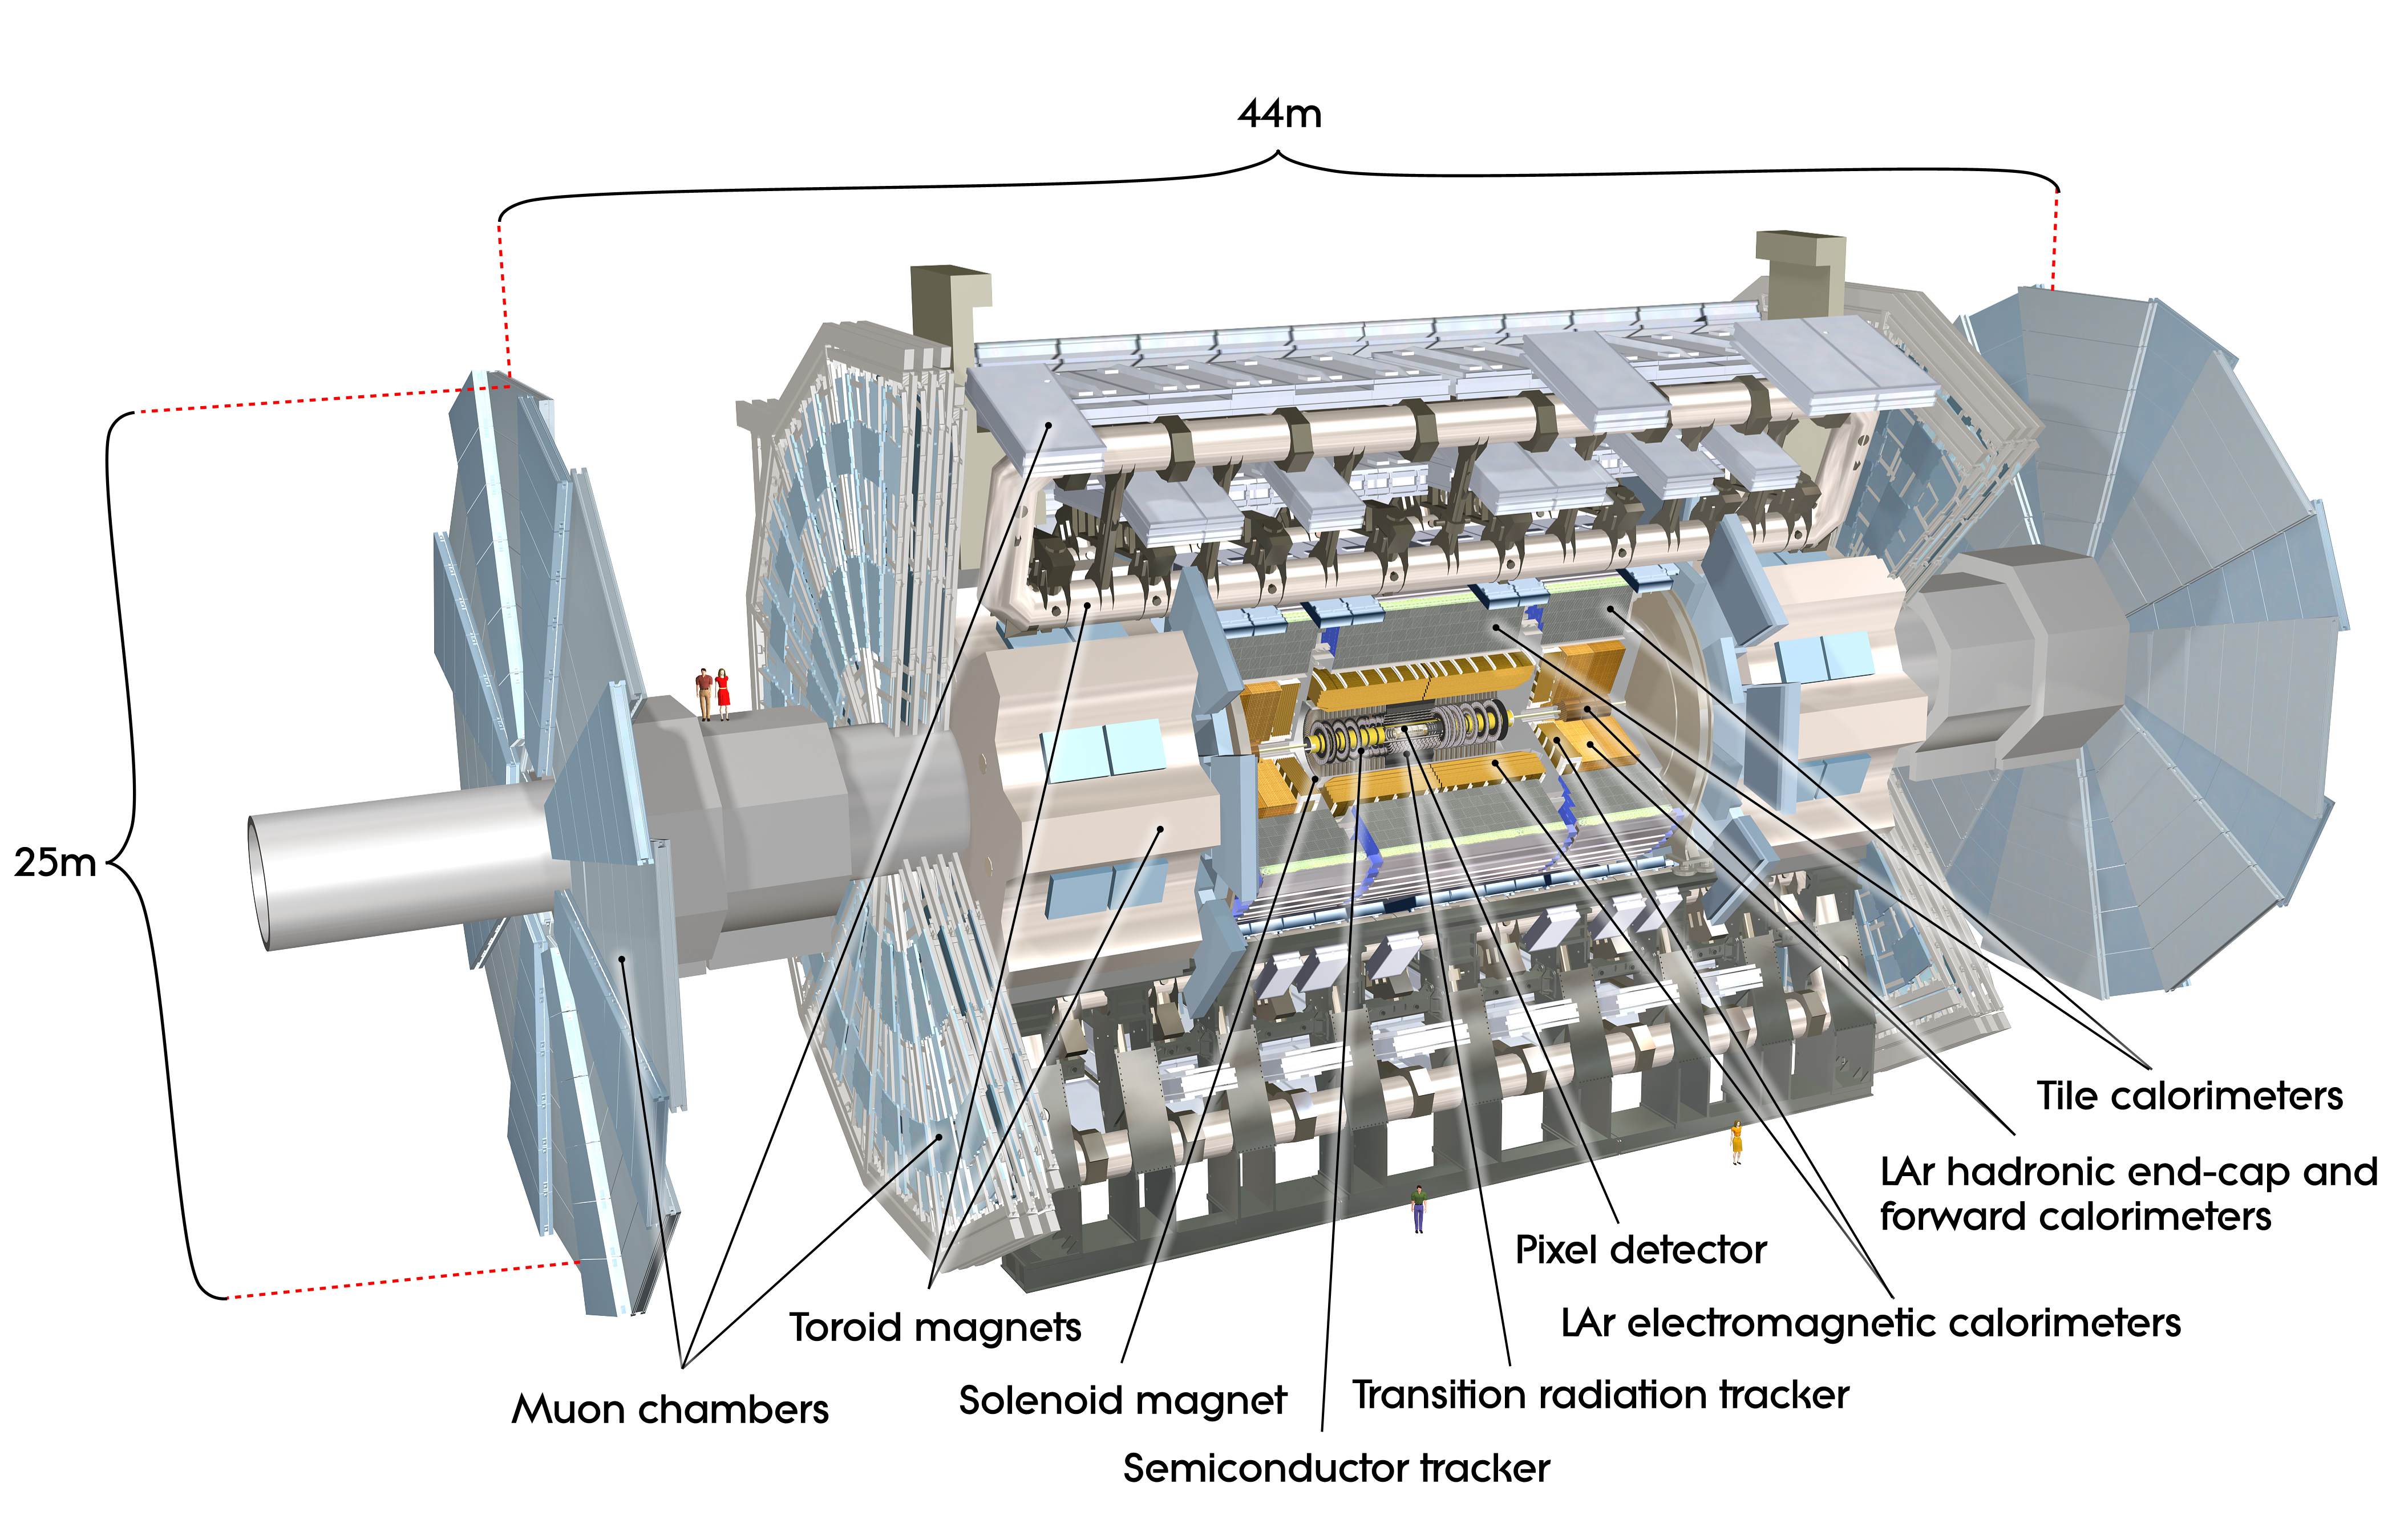
\includegraphics[scale=0.15]{figures_LHC/atlas-detector}
  \caption[Sketch of the ATLAS detector]{Sketch of the ATLAS detector and all its components including two average humans for scale.~\cite{Pequenao:1095924}}
  \label{fig:atlas}
\end{figure}

\subsection{The ATLAS coordinate system}

The ATLAS coordinate system is a right-handed and right-angled coordinate system with the $z$-axis pointing along the LHC's beam pipe. The corresponding transverse plane is defined by the $x$-axis pointing towards the ring's centre while the $y$-axis points upwards. The origin of the system is defined by the nominal point of interaction. The polar angle, $\theta$, is the angle between the $z$-axis and the $x$-$y$-plane and the azimuthal angle, $\phi$, is the angle between the $x$- and the $y$-axis.

Alternatively, as in this work, an event's topology is described by the azimuthal angle $\phi$, the pseudo-rapidity, $\eta$, and the transverse momentum, \pT. The pseudo-rapidity replaces the polar angle and is defined as

\begin{equation}
\eta = \frac{1}{2} ln\left[ tan\left(\frac{\theta}{2}\right)\right] \approx \arctanh\frac{p_z}{E}.
\end{equation}

The transverse momentum is defined as

\begin{equation}
\pT = \sqrt{p_x^2 + p_y^2},
\end{equation}
where $p_x$ and $p_y$ are the momenta along the corresponding axes. 

The angular variables are defined within

\begin{equation}
\eta \in [-\infty,\infty],\,
\phi \in [-\pi,\pi].
\end{equation}


The shape of the ATLAS detector makes the cylindrical system the obvious choice. This comes with the additional benefit of a well defined transverse plane where the sum of all vectors in the final state should be zero because the initial state has no transverse momentum.



\subsection{Tracking detectors}

Tracking detectors are used to measure a charged particle's trajectory, momentum and charge value, of which two types are used in the ID of the ATLAS detector. The Pixel detector and the Semi Conductor Tracker (SCT) are silicon detectors and the Transition Radiation Tracker (TRT) is a straw-based tracking detector. For all detectors it holds true that they are surrounded by a magnetic field and cover a pseudorapidity range of $|\eta| < 2.5$. The magnetic field results in curved trajectories enabling an estimate of momentum and charge.\cite{leo}

Pixel detectors are based on ionisation of charged particles in the semiconductor material. The induced charge is picked up by the detector's pixels providing a position information. To provide a 3-dimensional trajectory the pixel-chips are ordered in 4 layers around the beam pipe where the layer closest to the point of interaction, called Insertable B-Layer (IBL), was added in 2015. It is located only \SI{3.3}{\centi \metre} from the beam pipe and allows to detect vertices very close to the interaction point mainly originating from \Pbottom-quarks giving the layer its name.~\cite{pixel_run2}

The SCT as a silicon microstrip detector is the second silicon-based tracker immediately following on the pixel detector. It consists of modules of four silicon strip sensors organised in four barrel layers and eighteen planar endcap disks.

The TRT is structured in straw tubes each tube being an individual drift chamber with a strong potential difference due to negatively charged walls. The tubes are filled with a gas mixture (\ce{Xe} or \ce{Ar}) causing transversing charged particles to ionize and then by accelerated to the walls. A cascade is initiated and a measurable signal in the potential difference is measured. 
Between the tubes material is inserted resulting in transition radiation. This radiation has a cross section way higher for electrons than for other particles over a wide range of energy thus adding particle information to the track information provided by the TRT.

A particle being detected in a layer of the ID is called a hit. The record of hits gives an estimate on the particle's trajectory and can thereby also provide information on the vertex the particle originates from. This vertex information is worth mentioning as for a an experiment with an event count as large as the ATLAS experiment's events interfere and information from so called pileup events can affect the event's information. As pileup originates from different events it can be separated from the event of interest by separating the vertices.

\subsection{The ATLAS calorimeter system}

The ATLAS calorimeter system is divided into three main parts. The electromagnetic (EM) calorimeter, comprising a barrel and two end-caps, and the hadron calorimeter, built by a tile calorimeter, consisting of a a barrel and two so called "extended barrels", and the hadron end-caps. The third part is the forward calorimeter which additionally focuses on electromagnetic interaction. The tile calorimeter is scintillator-based apart from that the main part of the calorimeter system is based on liquid argon. The components cover a pseudorapidity range of $|\eta| < 4.9$

Calorimeters determine a traversing particle's energy by exploiting the formation of particle showers.~\cite{wermes} Due to inelastic collisions in the detector's material, the energy of the original particle is distributed on a cascade of secondary particles finally stopped by ionization. The resulting charge or photons can be measured as an estimate of the initial energy.

Electromagnetic calorimeters exploit the energy loss of electromagnetically interacting particles in matter. Mainly photons and electrons loose their energy based on pair production and Bremsstrahlung respectively. The energy loss initializes a cascade of particle decays called an electromagnetic shower. The decay stops when the shower particles do not hold sufficient energy for a decay anymore. The energy of the final state shower particles is picked up by the detector representing the initial particle's energy.
The ATLAS ECAL is a sampling calorimeter, built of two alternating layers of absorber and detection material. In the absorber the showers are induced to subsequently be detected in the detection layers.


As the ECAL uses electromagnetic showers the hadronic calorimeter depends on hadronic shower evolution. Hadronic showers are initialized due to ionisation or strong interaction with the material's nuclei. If the resulting particles still interact with the material a shower evolves.
The hadronic tile calorimeter is made of alternating layers of steel absorbents and scintillators covering a pseudorapidity range of $|\eta| < 1.6$.
The hadronic endcap calorimter (HEC) is liquid argon-based and covers $1.4 < |\eta| < 3.1$
Due to the larger size of hadronic showers the HCAL occupies more detector space than the ECAL.


\subsection{The Muon spectrometer}

The second tracking detector of ATLAS is the muon spectrometer which is the outermost part of the detector. The task of the spectrometer is to detect charged particles traversing the calorimeter without being stopped or deploying their complete energy, and to do both collect trigger information and information on trajectory and momentum. Due to these two tasks the spectrometer is bifid with the first part being the trigger chamber covering a range of $|\eta|<2.4$, followed by the high-precision chamber with a range of $|\eta|<2.7$. The main detector's support feet cause a further gap at about $\phi = \ang{300}$ and $\phi = \ang{270}$.

Normally the only charged particles left to be detected in the muon spectrometer are muons giving the component its name and allowing to provide good trigger information for researches interested in muons in the final event topology.





\subsection{Particle Detection in the ATLAS detector}

This section focuses on the detection and distinction of different particle types in the ATLAS detector. The capability and combined information of the detector components is introduced giving an explanation of the general working principle and also of the characteristics defining the events in this work. Figure \ref{fig:atlas_sketch} gives an overview of typical particle interactions and detections.

In order to reconstruct the particles in an event low level information is gathered using the direct detector output and then associated to the higher level particle information.

The information from the ID is called a track and contains not only the trajectory but also tells how consistently a track holds hits in every layer. A track offers momentum and charge information and can be associated with a vertex and a possible energy deposition in a calorimeter. 
The vertex reconstruction arising from the track information allows to define a primary vertex defined by the highest sum of squared transverse momenta while additional vertices are identified as pileup vertices.
Secondary vertices originating from tracks connected to the original vertex can be collected to identify short-lived particles.

The calorimeter data is summarised in clusters. Clusters are neighboring calorimeter cells with energy depositions significantly higher than the expected noise. A cluster is formed around a high energy deposition and can be associated to hadrons or jets or even to a corresponding track.

In the following the higher order objects reconstructed from this basic information are introduced to then explain the decisions made in the event selection for the \tW channel.

\begin{description}
\item[Electrons] 
are constructed from energy deposits in the EM associated with ID tracks.
To improve the decision rule, a likelihood object quantity is constructed from the shape and the ratio of the calorimeter to tracker response, and a set of further variables suitable for a better discriminant. There are three settings for the likelihood object namely tight medium and loose depending on how restrictive the analysis is.
Lastly an isolation quantity is defined based on cones around the track and the EM deposit to further decimate background and fake electrons.~\cite{ATLAS-CONF-2016-024}
\item[Jets] are cones of particles originating from the common hadronisation of a quark or gluon. In the detector they are reconstructed using 3-dimensional topological clusters of calorimeter energy.~\cite{Aad:2016upy} In addition to this there is further information that can be associated to jets, {i.e.}, an ID track or a vertex using a jet-vertex-tagger to minimize the impact of pile-up events and to associate to secondary vertices. For reconstruction the \antikt algorithm was used.~\cite{Cacciari:2008gp}
\item[Muon] reconstruction uses MS hits matched with ID tracks. The choice can be further specified by applying an identification cut based on MS/ID agreement and integrity of MS hit response. As for electrons isolation can be required.~\cite{Aad:2016jkr}
\item[\Pbottom-jets] are jets originating from the decay of a \Pbottom-quark and therefor a strong discriminant for events containing a \Ptop decay. The process of identifying a \Pbottom-jet is called \Pbottom-tagging and uses a multivariate discriminant. The topology of \Pbottom-jets is distinguishable from other jets due to for example clear secondary vertices, vertex alignment of a primary, a secondary \Pbottom-vertex and a tertiary \Pcharm-vertex, the decay length, and the characteristic energy scale.~\cite{Aad:2110203, ATL-PHYS-PUB-2016-012}
\item[Missing transverse momentum]
arises from momentum imbalance in the transverse plane. Momentum in the transverse plane should be preserved due to it being perpendicular to the beam axis and imbalance is an indicator for neutrinos escaping the detector. It is calculated using two contributions, one being signals from fully reconstructed and calibrated particles and the other one is information from reconstructed charged particle tracks. ~\cite{Aaboud:2018tkc}  
\end{description}

In addition to this the ATLAS trigger system has to be mentioned. Although potentially deserving a chapter of its own for this work it is sufficient to just state  and briefly explain trigger information.

Triggers are used to filter events before the actual event selection is taken into account. Given the incredible luminosity of the LHC such a preselection is important to minimize the data actually processed by the more complicated analysis algorithms and selection schemes.
The ATLAS trigger system consists of three triggers, namely the Level 1 (L1), Level 2 (L2), and the Event Filter (EF) where L2 and EF are generally referred to as the High-Level Trigger (HLT).

The L1 is is completely hardware-based and its decision making process is motly based on information from the calorimeter and the muon trigger chambers. The decision step relies on high-\pT objects and their multiplicity in an event while also considering missing transverse momentum and the beam condition to provide a first and very broad event selection.

The HLT is based on software and takes the L1 events as input. L2 defines so called regions of interest (ROI) as those regions in the angular plane where the trigger objects for L1 were detected and applies further trgger cuts to these objetcs.
The EF fully analyzes the event based on the complete information available.

This trigger information can be used for event selection making sure that certain final state objects are dominant in the topology and also to just apply a first, broad selection.



\begin{figure}[htbp]
  \centering
  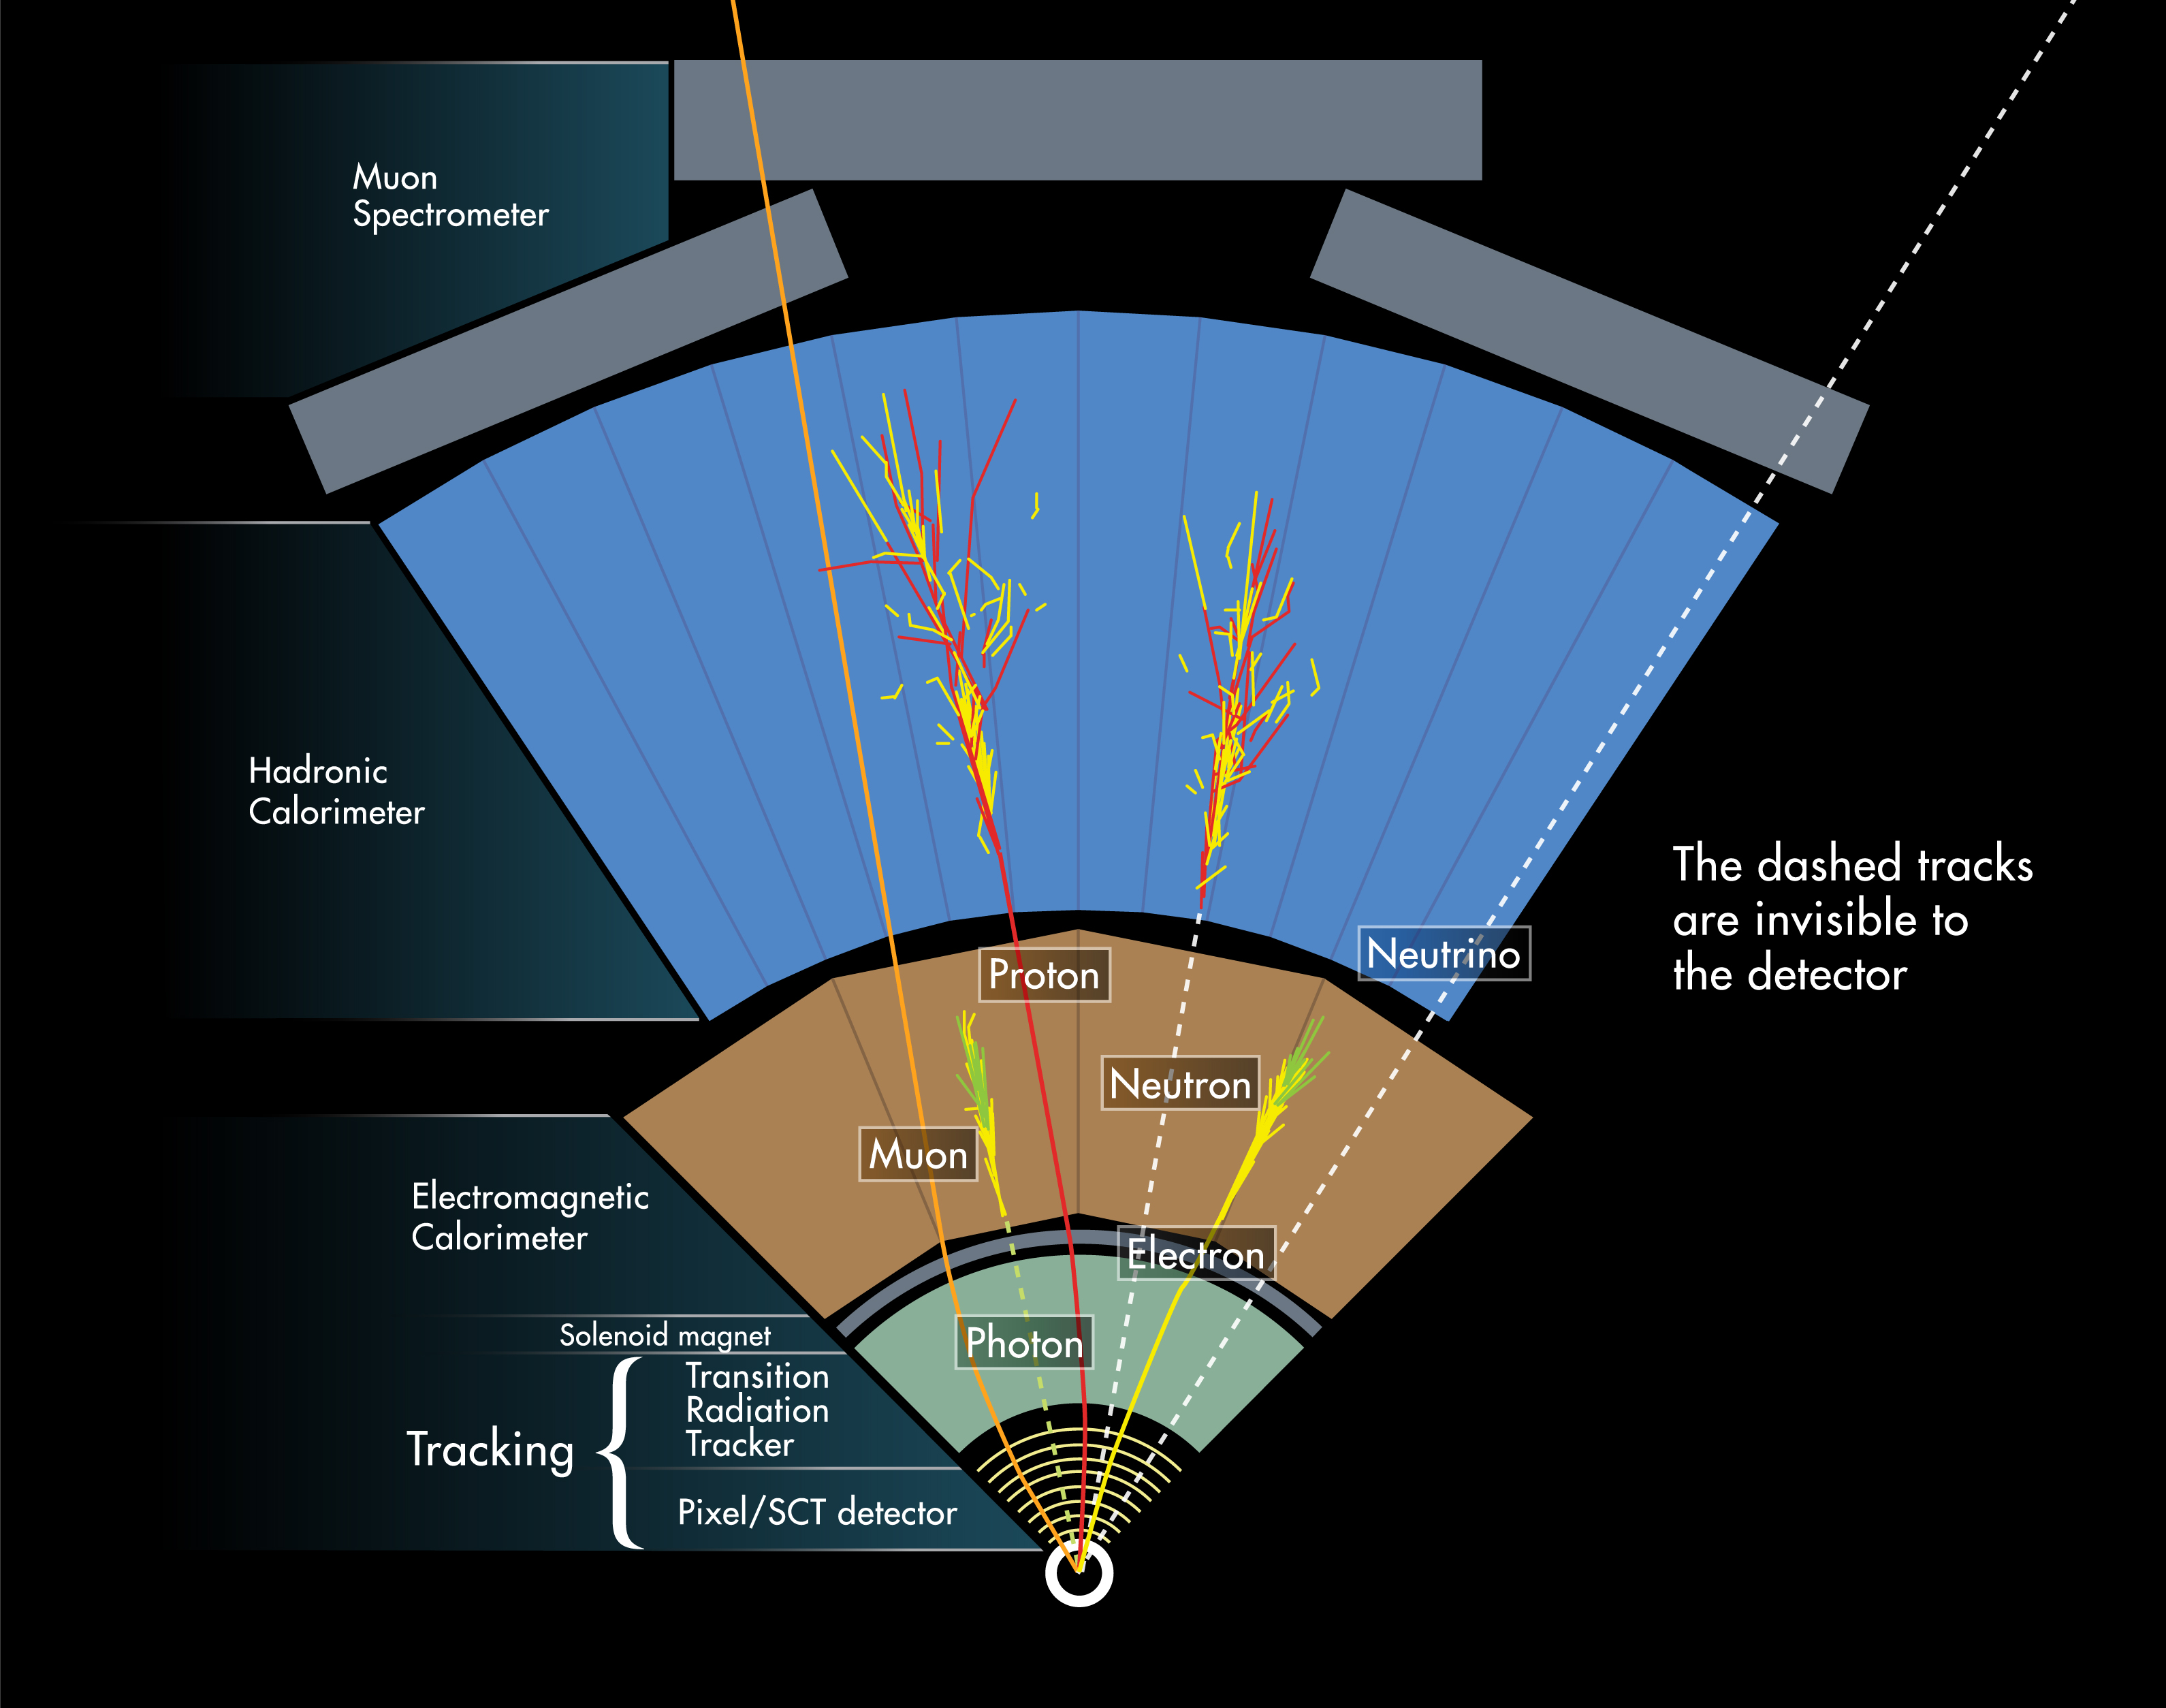
\includegraphics[scale=0.6]{figures_LHC/atlas-abstract}
  \caption[Scheme of the ATLAS-detector's detection procedure]{Scheme of the ATLAS-detector showing examples of typical particle detections. \cite{Pequenao:1095924}}
  \label{fig:atlas_sketch}
\end{figure}


%A Monte Carlo simulation is a statistical simulation of a possibly deterministic system. 

%detector simulation runs on top of Monte Carlo simulation

%Simulations are based on cross sections which can be calculated and measured in units of \textsc{barn} where \SI{1}{\barn} = \SI{1e-28}{\square \metre}

%Simulations heavily rely on quantities than can both be calculated and measured in an experiment thus allowing for predictions and also for  controlling the theoretical values.
%In high energy particle physics there are mainly two such quantities cross section and branching ratio0

%In collisions not only the valence quarks but also the sea quarks are relevant which can be explained by the valence quarks radiating gluons and quark antiquark pairs with no net flavour change.also explains the mass

\section{tW event selection}

The process that this work focuses on is the \tW-channel in the dilepton decay mode, and its most relevant background process: top-quark pair-production, \ttbar.
Other backgrounds for the \tW channel are reduced by applying an event selection:


\begin{itemize}
\item A single electron or muon trigger
\item Electrons: tightly identified, isolated, \ET > \SI{26}{\giga \electronvolt}
\item Muons: tight isolation, \pT > \SI{26}{\giga \electronvolt}
\item A pair of leptons with opposite electric charge
\item Leading lepton \pT > \SI{27}{\giga \electronvolt}
\item Veto for a third lepton \pT > \SI{20}{\giga \electronvolt}
\item A lepton must match the trigger
\item At least one jet with: \pT > \SI{25}{\giga \electronvolt}, $|\eta|$ < \num{2.5}, tagged at \num{77} \% working point
\end{itemize}

After this preselection the events are categorized in regions based on the jet and \Pbottom-jet multiplicities. For this work the region with exactly two \Pbottom-tagged jets was used, denoted as \texttt{2j2b}. This region has especially high impact from the NLO interference with a \ttbar final state.

\section{Monte Carlo simulation}

A Monte Carlo simulation is a computer based stochastic calculation of a process that in principle could be deterministic. However, the problem and the amount of statistics suggest a stochastic approach.

Monte Carlo, in the context of the ATLAS experiment, is the simulation of physics processes used to calibrate the performance of the detector and to compare model and measurement. As for for this work, the classifying tools and event selection rules are tested and tuned based on simulations to achieve a better understanding of what efficiencies are to be expected in a data analysis. This provides the truth labels to an event that is needed for supervised learning, see section \ref{chp:ml}, and cannot be provided by data.

A simulation has to be based on quantities that can not only be calculated from theoretical models but also measured during the experiment, because the models should reflect reality in terms of physics processes and detector effects. In collider physics, predictions are mainly based on  the cross-section of an interaction stating how high the probability for certain interaction is. In addition, the decay width of a particle is needed to describe how particles generated in an interaction behave in the detector system.

A proton-proton collision is modeled by describing the protons as a sea of partons, {i.e.}, the gluons and quarks their momentum is carried by, and then calculating the cross-sections for these partons to interact. The technique of seeing the collision as an interaction of two individual partons while decoupling these interactions from the parton interactions in the individual protons is called factorization.
For a parton carrying a fraction $x$ of the proton's momentum for a center-of-mass energy, $\hat{s}$, the cross-section, $\sigma(p_1 p_2 \rightarrow X)$, to create a final state $X$ can be described as:
%
\begin{equation}
	x_i = \frac{p_{parton,i}}{p_{proton}}, 
\end{equation}
%
%
\begin{equation}
	\hat{s} = x_1 x_2 s,
\end{equation}
%
%
\begin{align}
	\sigma ( p_1 p_2 \rightarrow X ) = \sum_{i,j = \Pquark, \APquark, \Pgluon} \int dx_i dx_j f_{i/p_1} ( x_i, \mu^2 ) f_{j/p_2} ( x_j, \mu^2 ) \cdot \hat{\sigma}_{ij} ( ij \rightarrow X; \hat{s}, \mu^2 ).
	\label{eq:factorisation}
\end{align}
%
There are two quantities in equation~\ref{eq:factorisation} not yet explained.
The parton density function (PDF), $f_{i/p_m} ( x_i, \mu^2 )$ denotes the probability of a parton with a certain momentum fraction, $x_i$, in the proton $k$ takes part in the hard scattering.
The PDF is independent of the collision and has to be gained from experiments rather than through calculations.

The second quantity $\mu$ is the so called factorization scale. It describes to which degree the interactions of the partons in the proton can be neglected. It is an arbitrary scale determining the precision of the simulation to some degree.

\subsection{ATLAS simulation}

The MC simulation for the ATLAS detector is generated in two steps~\cite{atlasmontecarlo}.
In the first step the actual collision is simulated, defining the particles in the final state. The underlying algorithm is called Monte Carlo event generator.

Secondly, the response to these particles is simulated by the detector simulation allowing objects to be reconstructed from the event similar to actual data gaining a comparison on every level of reconstruction.

Furthermore, a set of different options and generators can be chosen for the simulation. Examples would be how a parton shower is simulated or to which degree multi-parton interaction is taken into account.

\subsection{Systematic uncertainties in Monte Carlo simulations}
\label{sec:systmc}

Simulations, as described earlier, have to be based on certain assumptions about the input parameters. This is especially true in those cases for which the theory does not offer a precise result. This results in systematic uncertainties arising from the simulations, which should be taken into account when performing an analysis.
In those cases different Monte Carlo samples are produced, each representing a different assumption about the initial parameters; showing first of all how the data should behave with these scaled parameters and allowing to test whether the systematic or the original sample fits better to the data. 
These samples of Monte Carlo will just be referred to as systematics in this work.

Usually the simulations use the leading order diagrams.
When next-to-leading order diagrams become relevant, the simulation sometimes has to be adapted resulting in different samples for different orders.
This work focuses on the \tW and \ttbar events interfering at NLO as described in section~\ref{chp:tw}
The total NLO amplitude is the sum of the of singly resonant diagrams and all doubly resonant diagrams:

\begin{align}
\Aamp = \Atw + \Att.
\end{align}

Calculating the cross-section requires the square of this amplitude:

\begin{align}
|\Aamp|^2 &= |\Atw|^2 + 2 \mathcal{R} \{ \Atw \Att^{\ast} \} + |\Att|^2, \\
&\equiv \Samp + \Iamp + \Damp.
\end{align}

The Diagram Removal approach is used as a nominal sample, denoted as DR, is used. It fully removes the \Att amplitude and thus both the pure \ttbar contribution as well as the interference term vanish.

\begin{align}
| \ADR |^2 = \Samp
\end{align}

Alternatively the Diagram Subtraction or DS can be used, which is in this work represented by the systematics sample. It introduces a gauge invariant term that cancels the \ttbar contribution and in a simplified way, can be written as

\begin{align}
| \ADS |^2 &= \Samp + \Iamp + \Damp - \widetilde{\Damp},\\
&\approx \Samp + \Iamp.
\end{align}

The nominal samples were produced using a full ATLAS detector simulation implemented in \GEANTfour and the systematic samples were mostly simulated using \ATLFASTtwo~\cite{geant, atlfast}. The systematic samples used in this thesis were produced using \GEANTfour as a DS sample requires a full simulation.

The events were generated by \POWHEG\PYTHIA8~\cite{pythia}.

%---------------------------------------------------------------------
